\section{Contenu technique}
    \subsection{Cas d'utilisation}
    Le premier cas d'usage (figure~\ref{fig.casUsage1}) consiste en une application d'horaire spécialement conçue pour les étudiants en génie de l'Université de Sherbrooke. La simplicité, la mobilité et l'accessibilité de la gestion d'horaire en sont les caractéristiques principales. En effet, l'application mobile permet à l'étudiant de visualiser son horaire et de recevoir des notifications en cas de changement d'horaire. L'application propose plusieurs paramètres pour personnaliser la réception de notifications
    
    \begin{figure}[p] \centering
%        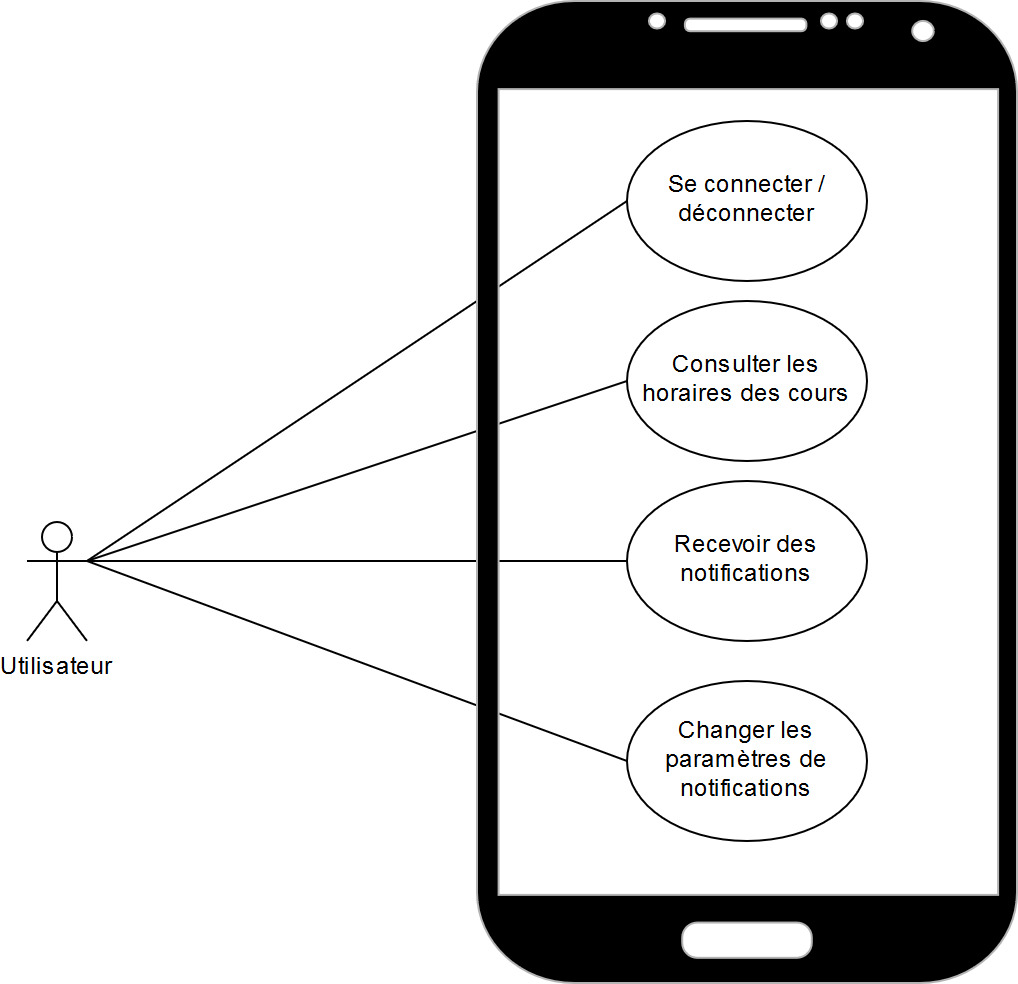
\includegraphics[width=\textwidth]{Figures/casUsage1}
        \begin{tikzpicture}\tikzstyle{every node}=[font=\small]
  \node[inner sep=0pt] (iphone) at (7,0) {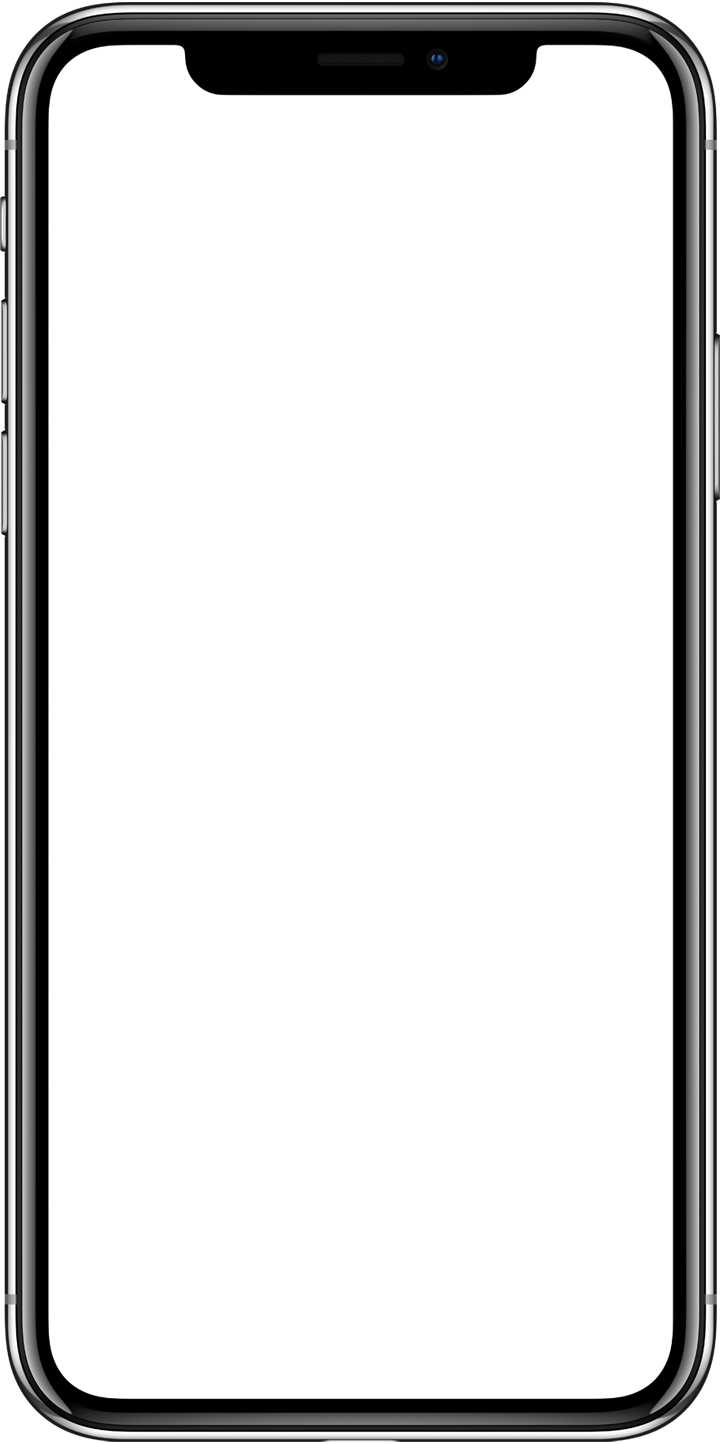
\includegraphics[width=.35\textwidth]{Figures/iphone.png}};
  \node[graduate, minimum size=1.5cm] (user) at (0,0) {Utilisateur};
  \node[draw, ellipse, align=center] (connect) at (7,3) {Se connecter \\ Se déconnecter};
  \node[draw, ellipse, align=center] (schedule) at (7,1) {Consulter les \\ horaires des cours};
  \node[draw, ellipse, align=center] (notif) at (7,-1) {Recevoir \\ des notifications};
  \node[draw, ellipse, align=center] (param) at (7,-3) {Changer \\ les paramètres de \\ notifications};
\draw (user.east) -- (connect.west);
\draw (user.east) -- (schedule.west);
\draw (user.east) -- (notif.west);
\draw (user.east) -- (param.west);
\end{tikzpicture}
        \caption{Diagramme du premier cas d'usage de l'application}
        \label{fig.casUsage1}
    \end{figure}

    Le deuxième cas d'usage (figure~\ref{fig.casUsage2}) consiste en une plateforme de communication sociale entre les étudiants et les professeurs. Présentement, il n'y a que le changement d'horaire qui est lié à cette forme de communication, mais l'infrastructure de l'application permet l'intégration de notifications tierces. À cet effet, la communication d'éléments jugés importants par l'équipe professorale peut être effectuée via le centre de notifications de l'application dans le but de divulguer cette information aux étudiants concernés. On distingue trois types d'utilisateurs :
    \begin{description}
        \item[Un(e) étudiant(e) de l'université de Sherbrooke] Il s'agit des utilisateurs les plus nombreux. On cherchera à maximiser la transparence de l'application pour ces utilisateurs afin qu'ils puissent se connecter et se déconnecter, consulter les horaires de cours, recevoir les notifications et modifier les paramètres associées à ces mêmes notifications sans obtenir de détails sur le fonctionnement interne du système.
        \item[Un administrateur du système] Il devra s'authentifier, aura accès à toutes les permissions des utilisateurs et sera en mesure d'envoyer des notifications à l'application.
        \item[L'équipe de notifications] Le système se voulant être distribué et modulaire, un type d'utilisateur est réservé pour les autre équipes de projet qui sont susceptibles de gérer des notifications et de les envoyer à notre application. Ce type d'utilisateur particulier devra s'authentifier comme les autres et n'aura accès qu'à une partie restreinte du système, laquelle lui accorde la permission d'envoyer des notifications.
    \end{description}
        
    \begin{figure}[p] \centering
%        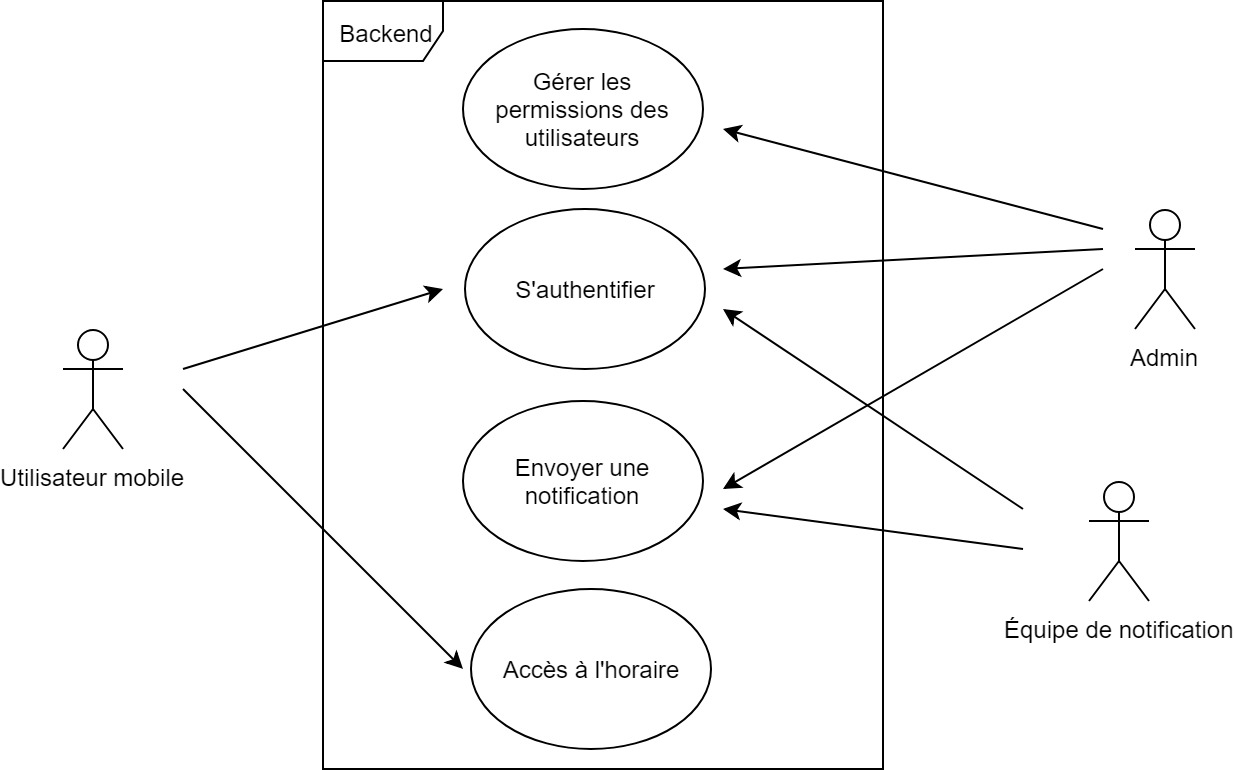
\includegraphics[width=\textwidth]{Figures/casUsage2}
        \begin{tikzpicture}\tikzstyle{every node}=[font=\small]
  \node[graduate, minimum size=1.5cm] (user) at (0,0) { Utilisateur mobile};
  \node[businessman, mirrored, minimum size=1.5cm] (admin) at (10,2) { Administrateur};
%%%%%%%%%%%%%
  \node[jester, mirrored, minimum size=1.5cm] (team) at (10,-2) { Équipe de notification};
  \node[draw, ellipse, align=center] (perm) at (5,3) { Gérer les \\  permissions des \\  utilisateurs};
  \node[draw, ellipse, align=center] (auth) at (5,1) { S'authentifier};
  \node[draw, ellipse, align=center] (notif) at (5,-1) { Envoyer une \\  notification};
  \node[draw, ellipse, align=center] (access) at (5,-3) { Accès à l'horaire};
%%%%%%%%%%%%%
\draw[-latex] (user.east) -- (auth.west);
\draw[-latex] (user.east) -- (access.west);
\draw[-latex] (admin.west) -- (perm.east);
\draw[-latex] (admin.west) -- (auth.east);
\draw[-latex] (admin.west) -- (notif.east);
\draw[-latex] (team.west) -- (auth.east);
\draw[-latex] (team.west) -- (notif.east);
%%%%%%%%%%%%%
\draw (2,-4) -- (2,5) -- (8,5) -- (8,-4) -- (2,-4);
\node[anchor=north west, draw] at (2,5) {{\bfseries Backend}};
\end{tikzpicture}
        \caption{Diagramme du second cas d'usage de l'application}
        \label{fig.casUsage2}
    \end{figure}

    \subsection{Design patterns utilisés}
    La structure du code de ce projet suit plusieurs \emph{design patterns} différents. Pour ce qui est du système dans son ensemble, le \emph{pattern} \emph{Model View Controller} a été appliqué : l'application mobile fait office de vue en présentant l'information dans son interface, la base de donnée est le modèle qui contient les données et communique à l'aide d'entités avec le serveur. Le backend fait le lien entre la vue et le modèle en tant que contrôleur à l'aide de \emph{data objects} \emph{sérialisés} en JSON.

    Concernant le backend, l'utilisation du \emph{framework} Spring et son fonctionnement par annotations nous obligent à utiliser l'\emph{injection de dépendances} avec les balises \code{@AutoWired} et le \emph{Singleton} (\code{@Bean}), car ce \emph{framework} va de pair avec l'injection de dépendances.

    Enfin, afin de permettre un filtrage des modifications d'horaire et de ne garder que des notifications d'événements à venir, nous avons mis en place un patron de spécifications (\emph{criteria pattern}). Ce patron se veut une chaîne de critères dans laquelle passent les événements et où seulement la sortie est utilisée pour envoyer les notifications. Les critères implémentés sont notamment l'élimination des événements passés et ceux qui sont plus d'un mois dans le futur.

    \subsection{Architecture du système}
    \begin{figure}[p] \centering
%        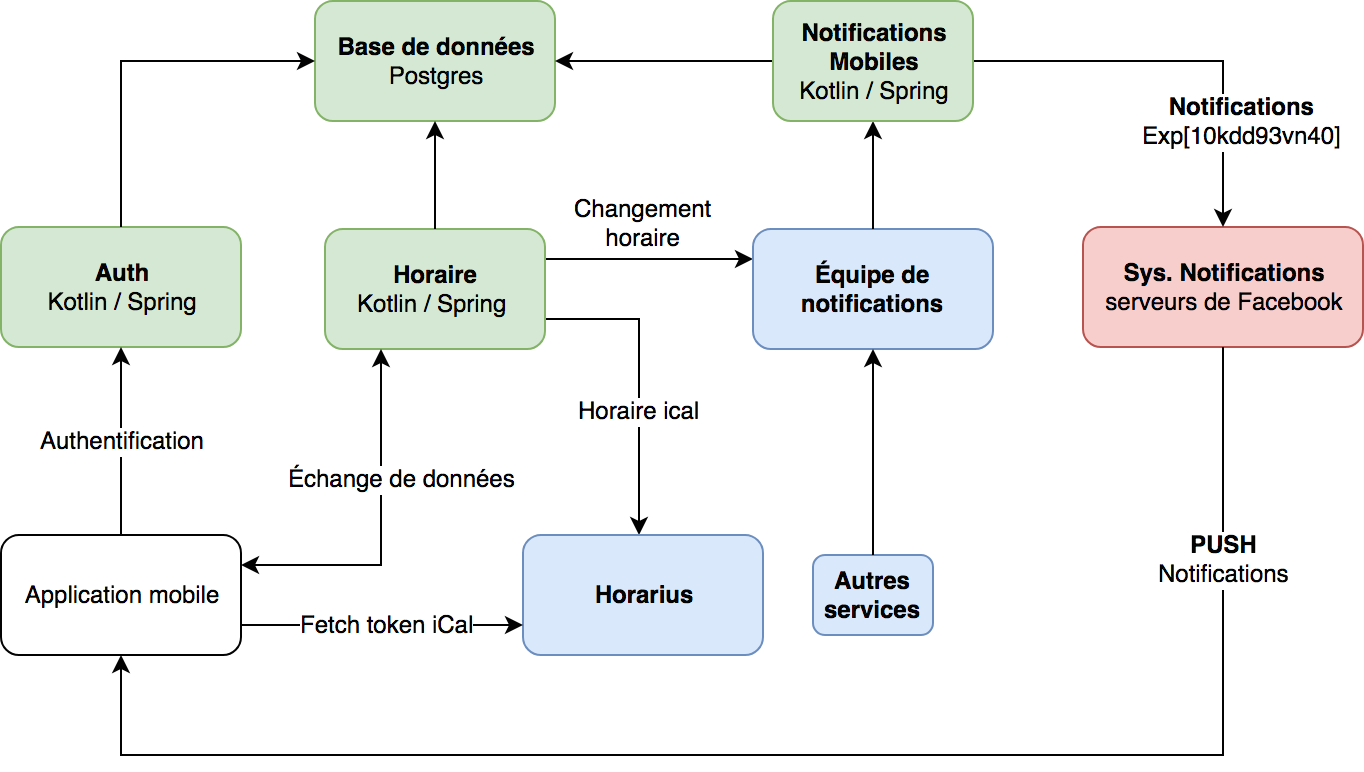
\includegraphics[width=\textwidth]{Figures/architectureSysteme}
        \begin{tikzpicture}\tikzstyle{every node}=[font=\small]
%%%%%%%% Colours %%%%%%%%
\definecolor{greenUML}{HTML}{D5E7D5}
\definecolor{blueUML}{HTML}{DAE8FB}
\definecolor{redUML}{HTML}{F8CECD}
%%%%%%%% White %%%%%%%%
  \node[draw, align=center, rounded corners, fill=greenUML] (app) at (0,0) {Application \\ mobile};
%%%%%%%% Green %%%%%%%%
  \node[draw, align=center, rounded corners, fill=greenUML] (auth) at (0,3) {\bf Auth \\ Kotlin/Spring};
  \node[draw, align=center, rounded corners, fill=greenUML] (db) at (3,5) {\bf Base de données \\ Postgres};
  \node[draw, align=center, rounded corners, fill=greenUML] (horaire) at (3,3) {\bf Horaire \\ Kotlin/Spring};
  \node[draw, align=center, rounded corners, fill=greenUML] (notif) at (9,5) {\bf Notifications \\ \bf mobiles \\ Kotlin/Spring};
%%%%%%%% Blue %%%%%%%%
  \node[draw, align=center, rounded corners, fill=blueUML] (team) at (9,3) {\bf Équipe de \\ \bf notifications};
  \node[draw, align=center, rounded corners, fill=blueUML] (autres) at (9,0) {\bf Autres \\ \bf services};
  \node[draw, align=center, rounded corners, fill=blueUML, minimum height=2\baselineskip] (horarius) at (6,0) {\bf Horarius};
%%%%%%%% Red %%%%%%%%
  \node[draw, align=center, rounded corners, fill=redUML] (sysNotif) at (12,3) {\bf Sys.\ notifications \\ Serveurs de Facebook};
%%%%%%%%%%%%%%%%%%%%%
% App
\draw[-latex] (app.north) -- node[midway, fill=white] {Authentification} (auth.south);
\draw[-latex] let \p1 = (app.east), \p2 = (horarius.west) in
  (\x1, {\y1-5}) -- node[midway, fill=white] {Fetch token iCal} (\x2, {\y2-5});
% Autres
\draw[-latex] (autres.north) -- (team.south);
% Notif
\draw[-latex] (notif.west) -- (db.east);
\draw[-latex] (notif.east) -- (12,5) -- node[midway, fill=white, align=center] {\bf Notifications \\ \scriptsize Exp[10kdd93vn40]} (sysNotif.north); % sorry hardcoded
% Team
\draw[-latex] (team.north) -- (notif.south);
% Horaire
\draw[-latex] (horaire.north) -- (db.south);
\draw[-latex] let \p1 = (horaire.east), \p2 = (team.west) in
  (\x1, {\y1+8}) -- node[midway, fill=white, align=center] {Changement \\ horaire} (\x2, {\y2+8});
\draw[latex-latex] let \p1 = (horaire.south), \p2 = (app.east) in
  (horaire.south) -- node[midway, fill=white, align=center] {Échange de \\ données} (\x1, {\y2+5}) -- (\x2, {\y2+5});
\draw[-latex] let \p1 = (horaire.east), \p2 = (horarius.north) in
  (\x1, {\y1-8}) -- (\x2, {\y1-8}) -- node[midway, fill=white] {Horaire iCal} (horarius.north);
% Auth
\draw[-latex] (auth.north) -- (0,5) -- (db.west); % sorry hardcoded
% Sys Notifications
\draw[-latex] (sysNotif.south) -- node[midway, fill=white, align=center] {\bf PUSH \\ Notifications} (12,-1) -- (0,-1) -- (app.south); % sorry hardcoded
\end{tikzpicture}
        \caption{Diagramme de l'architecture du système}
        \label{fig.architectureSysteme}
    \end{figure}
    
    \noindent L'architecture du système (figure~\ref{fig.architectureSysteme}) est divisée en différentes sections :
    \begin{description}
        \item[Éléments bleus] Services internes à l'Université
        \item[Éléments rouges] Services externes à l'Université
        \item[Éléments verts] Services fournis par l'équipe DEGEL
    \end{description}

    \noindent Les services fournis par DEGEL sont les suivants :
    \begin{description}
        \item[Authentification] Module qui regroupe tout ce qui touche de près ou de loin à l'authentification CAS et OAuth2. Ce module permet aussi de gérer les permissions des utilisateurs.
        \item[Horaire] Module qui s'occupe des communications avec \emph{Horarius}. Il gère les clés des utilisateurs et vérifie les changements d'horaire.
        \item[Notifications mobiles] Module qui reçoit les requêtes de l'équipe de notifications, lesquelles proviennent soit du module d'horaire, soit d'autres services externes. Il communique les notification aux utilisateurs par le biais des serveurs de Facebook (Expo).
    \end{description}

    \subsection{Modèle d'architecture logicielle}
        \subsubsection{Backend}
        \begin{figure}[p] \centering
%            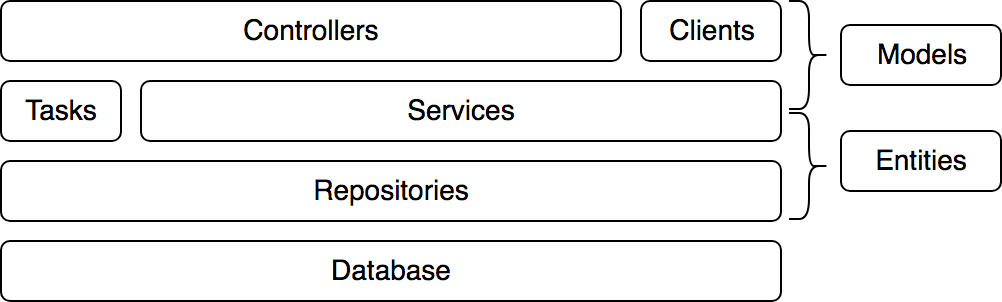
\includegraphics[width=\textwidth]{Figures/architectureBackend}
            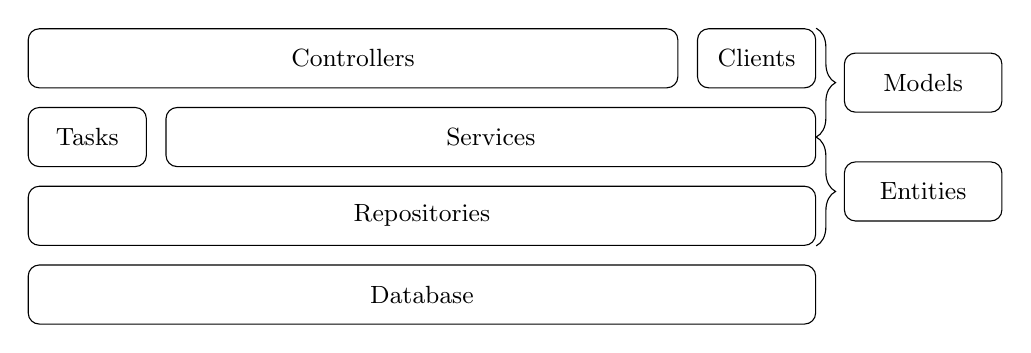
\begin{tikzpicture}%\tikzstyle{every node}=[font=\small]
\node[draw, rounded corners, minimum width = 10cm, minimum height = 0.75cm, anchor=west] (db) at (0,0) {Database};
\node[draw, rounded corners, minimum width = 10cm, anchor=west, minimum height = 0.75cm] (repo) at (0,1) {Repositories};
\node[draw, rounded corners, minimum width = 1.5cm, anchor=west, minimum height = 0.75cm] (tasks) at (0,2) {Tasks};
\node[draw, rounded corners, minimum width = 8.25cm, anchor=west, minimum height = 0.75cm] (services) at (1.75,2) {Services};
\node[draw, rounded corners, minimum width = 8.25cm, anchor=west, minimum height = 0.75cm] (controllers) at (0,3) {Controllers};
\node[draw, rounded corners, minimum width = 1.5cm, anchor=west, minimum height = 0.75cm] (clients) at (8.5,3) {Clients};
%%%%%%%%%%%
\draw [decorate,decoration={brace,amplitude=7pt}] (clients.north east) -- node[draw, rounded corners, minimum width = 2cm, anchor=west, minimum height = 0.75cm, midway, xshift=10pt] {Models} (services.east);
\draw [decorate,decoration={brace,amplitude=7pt}] (services.east) -- node[draw, rounded corners, minimum width = 2cm, anchor=west, minimum height = 0.75cm, midway, xshift=10pt] {Entities} (repo.south east);
\end{tikzpicture}
            \caption{Diagramme de l'architecture du backend}
            \label{fig.architectureBackend}
        \end{figure}
        
        \noindent Pour le backend, l'architecture choisie est le modèle en couches (figure~\ref{fig.architectureBackend}) :
        \begin{description}
            \item[Controllers] Ils définissent les \emph{endpoints} et les permissions associées à ceux-ci. Ils contiennent peu ou aucune logique d'affaire.
            \item[Services] C'est dans ceux-ci que la grande majorité de la logique d'affaire se retrouve. Ainsi, les tests se concentrent sur eux.
            \item[Repositories] C'est la couche ORM de l'application qui permet l'accès aux données persistantes.
            \item[Database] C'est l'instance qui s'occupe des données, Postgres dans notre cas.
        \end{description}

        \noindent Il y a également deux autres parties secondaires dans le modèle :
        \begin{description}
            \item[Tasks] C'est l'ensemble des tâches qui roulent en arrière-plan pour notamment aller chercher les modifications aux horaires.
            \item[Clients] Ceux-ci permettent de communiquer à d'autres services par HTTP.
        \end{description}

        Notons que les couches \emph{Services} et \emph{Repositories} communiquent entre elles avec des \emph{Entities} qui sont liées aux tables de la base de données. Ces entités sont transformées dans les services en \emph{Models} (et vice versa). Les services et les contrôleurs communiquent à l'aide de ces modèles.
        
        \subsubsection{Mobile}
        \begin{figure}[p]
%            \fbox{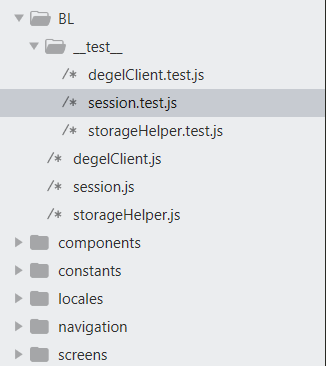
\includegraphics[width=0.5\textwidth]{Figures/architectureMobile}}
            \dirtree{%
.1 BL. 
.2 \_\_test\_\_. 
.3 /* degelClient.test.js. 
.3 /* session.test.js. 
.2 /* degelClient.js. 
.2 /* session.js. 
.2 /* storageHelper.js. 
.1 components. 
.1 constants. 
.1 locales. 
.1 navigation. 
.1 screens. 
}

            \caption{Arborescence de l'architecture mobile}
            \label{fig.architectureMobile}
        \end{figure}        
        
        Pour l'architecture mobile (figure~\ref{fig.architectureMobile}), l'ensemble tourne principalement autour des composantes de la partie vue de notre \emph{pattern} MVC :
        \begin{description}
            \item[Components] Parties visuelles réutilisables un peu partout dans l'application.
            \item[Screens] Les différentes vues qui seront présentées à l'utilisateur.
            \item[Navigation] L'agencement des différentes vues et les conditions pour passer de l'une à l'autre.
        \end{description}

        \noindent Il y également trois autres parties :
        \begin{description}
            \item[Constants] Utile pour regrouper les constantes de l'application, comme l'URL du serveur.
            \item[Locales] L'application étant localisée, tous les textes (français et anglais) s'y trouvent.
            \item[BL] La petite partie de logique d'affaire de l'application, notamment pour communiquer avec le serveur. C'est principalement cette partie qui sera testée.
        \end{description}
    
    \subsection{Modèle conceptuel de données}
    \noindent Le modèle reste plutôt simple : quatre entités indépendantes (figure~\ref{fig.entitesRequises}) requises par Spring :
    \begin{description}
        \item[flyway\_schema\_history] Contient l'histoire des migrations SQL effectuées.
        \item[oauth\_refresh\_token] Contient les jetons de rafraîchissement des utilisateurs.
        \item[oauth\_access\_token] Contient les jetons d'accès des utilisateurs.
        \item[oauth\_client\_details] Contient les informations sur les clients OAuth2 (qui sont l'application mobile et l'équipe de notifications).
    \end{description}
    
    \begin{figure}[p] \centering
%        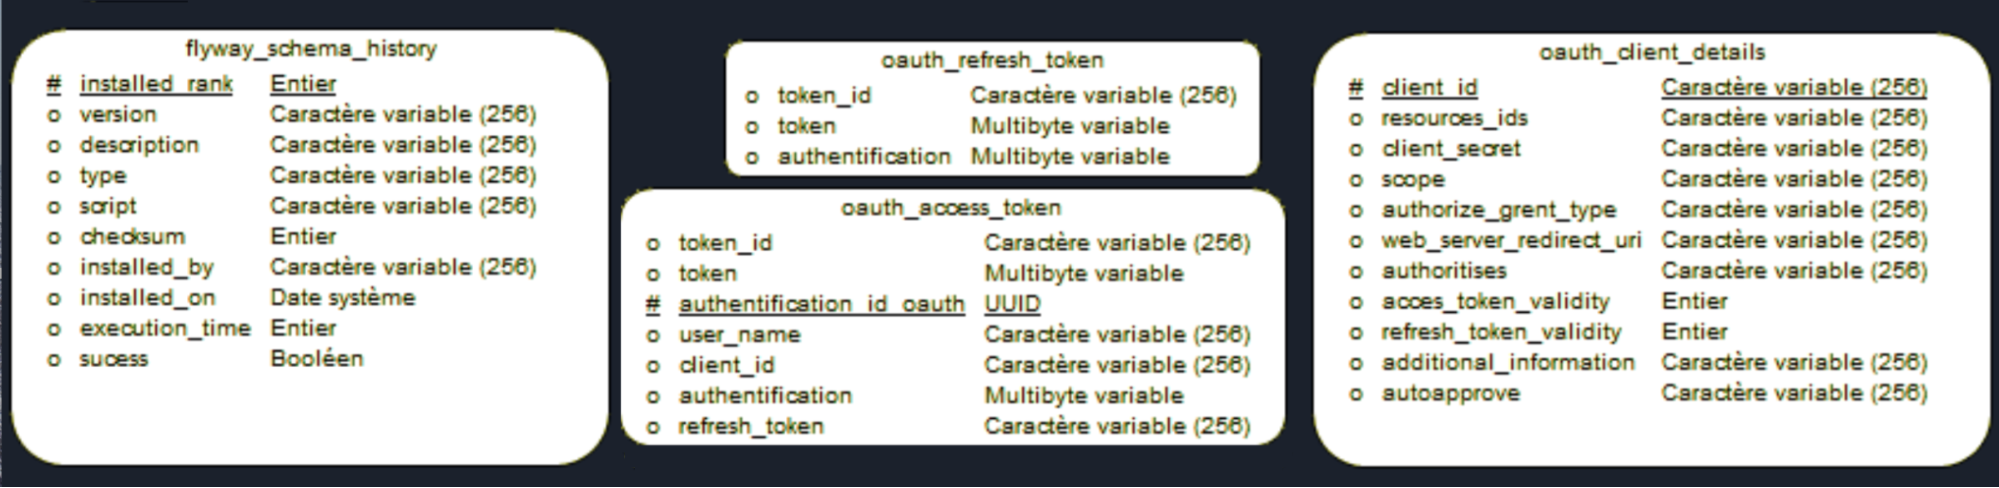
\includegraphics[width=\textwidth]{Figures/entitesRequises}
        \begingroup \renewcommand{\arraystretch}{1}
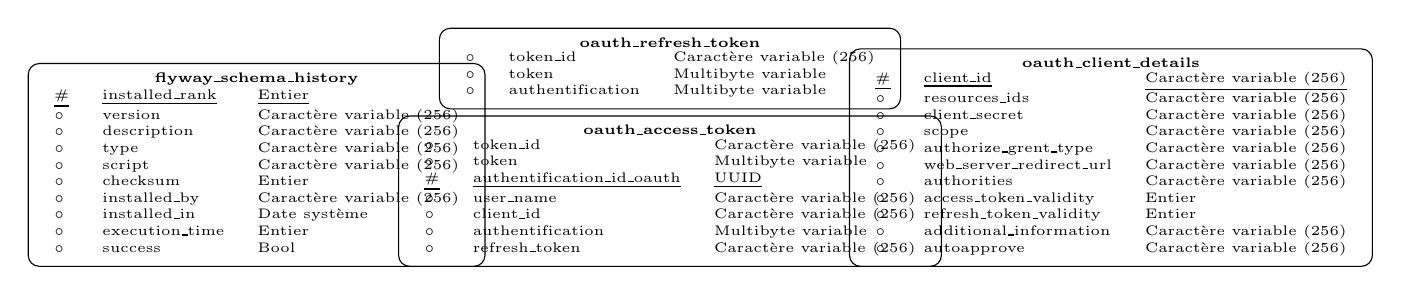
\begin{tikzpicture}\tikzstyle{every node}=[font=\tiny]
% flyaway_schema_history
  \node[draw, rounded corners, align=center, anchor=south] at (0,0)%
{%
  \bf flyway\_{}schema\_{}history \\
  \begin{tabular}{lll}
  \underline{\#} & \underline{installed\_rank} & \underline{Entier} \\
  $\circ$ & version & Caractère variable (256) \\
  $\circ$ & description & Caractère variable (256) \\
  $\circ$ & type & Caractère variable (256) \\
  $\circ$ & script & Caractère variable (256) \\
  $\circ$ & checksum & Entier \\
  $\circ$ & installed\_by & Caractère variable (256) \\
  $\circ$ & installed\_in & Date système \\
  $\circ$ & execution\_time & Entier \\
  $\circ$ & success & Bool
  \end{tabular}
};
% oauth_refresh_token
  \node[draw, rounded corners, align=center, anchor=south] at (5.25,2)%
{%
  \bf oauth\_refresh\_token \\
  \begin{tabular}{lll}
  $\circ$ & token\_id & Caractère variable (256) \\
  $\circ$ & token & Multibyte variable \\
  $\circ$ & authentification & Multibyte variable
  \end{tabular}
};
% oauth_access_token
  \node[draw, rounded corners, align=center, anchor=south] at (5.25,0)%
{%
  \bf oauth\_access\_token \\
  \begin{tabular}{lll}
  $\circ$ & token\_id & Caractère variable (256) \\
  $\circ$ & token & Multibyte variable \\
  \underline{\#} & \underline{authentification\_id\_oauth} & \underline{UUID} \\
  $\circ$ & user\_name & Caractère variable (256) \\
  $\circ$ & client\_id & Caractère variable (256) \\
  $\circ$ & authentification & Multibyte variable \\
  $\circ$ & refresh\_token & Caractère variable (256)
  \end{tabular}
};
% oauth_client_details
  \node[draw, rounded corners, align=center, anchor=south] at (10.85,0)%
{%
  \bf oauth\_client\_details \\
  \begin{tabular}{lll}
  \underline{\#} & \underline{client\_id} & \underline{Caractère variable (256)} \\
  $\circ$ & resources\_ids & Caractère variable (256) \\
  $\circ$ & client\_secret & Caractère variable (256) \\
  $\circ$ & scope & Caractère variable (256) \\
  $\circ$ & authorize\_grent\_type & Caractère variable (256) \\
  $\circ$ & web\_server\_redirect\_url & Caractère variable (256) \\
  $\circ$ & authorities & Caractère variable (256) \\
  $\circ$ & access\_token\_validity & Entier \\
  $\circ$ & refresh\_token\_validity & Entier \\
  $\circ$ & additional\_information & Caractère variable (256) \\
  $\circ$ & autoapprove & Caractère variable (256)
  \end{tabular}
};
\end{tikzpicture}
\endgroup
        \caption{Entités indépendantes requises par Spring}
        \label{fig.entitesRequises}
    \end{figure}
    
    \subsection{Persistance}
    \noindent L'ensemble des entités restantes sont nécessaires à l'application et sont toutes liées à l'utilisateur (figure~\ref{fig.persistance}).
    \begin{description}
        \item[users] Contient l'information de base sur chaque utilisateur (cip, actif, id).
        \item[authorities] Contient les rôles de chaque utilisateur. Un utilisateur peut avoir plusieurs rôle (ADMIN et USER par exemple).
        \item[notification\_token] Contient les divers tokens Expo de l'utilisateur. Un utilisateur a un token unique par appareil qu'il possède.
        \item[calendar] Contient les informations du calendrier de l'utilisateur dont notamment sa clé ical et le dernier calendrier qui a été retourné par horarius (pour faire les diff).
        \item[settings] Contient les préférences de l'utilisateur (une par colonne comme il n'y en pas beaucoup) notamment pour les notifications.
    \end{description}

    \begin{figure}[p] \centering
%        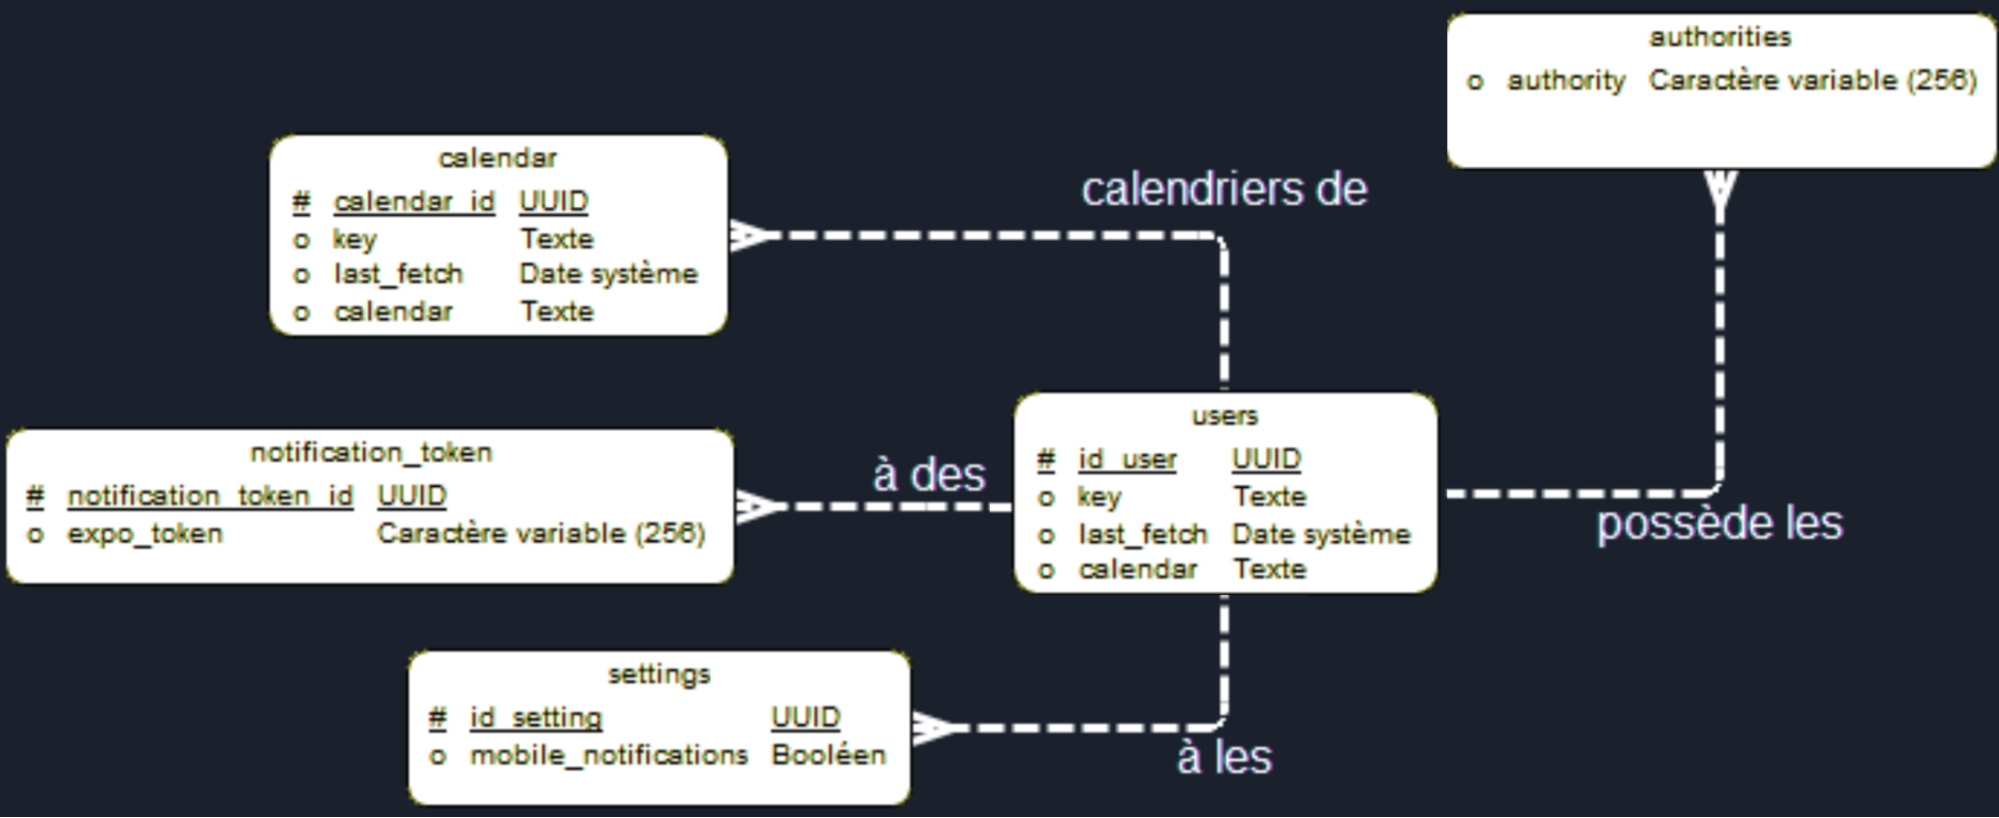
\includegraphics[width=\textwidth]{Figures/persistance}
        \begingroup \renewcommand{\arraystretch}{1}
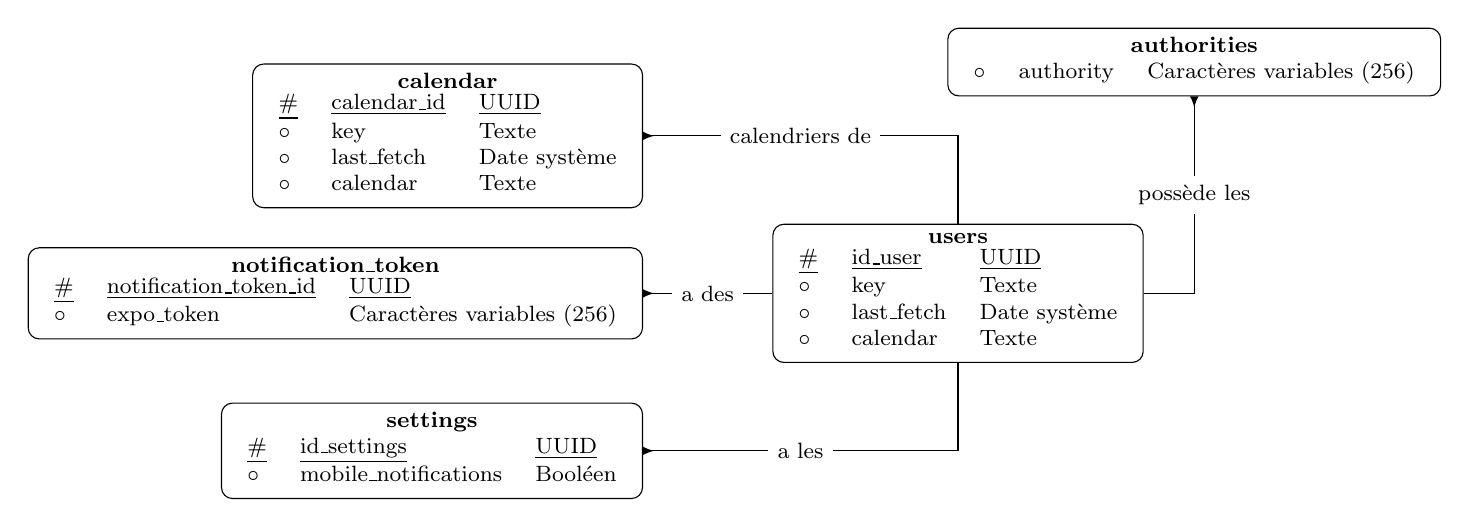
\begin{tikzpicture}\tikzstyle{every node}=[font=\footnotesize]
% users
  \node[draw, rounded corners, align=center] (users) at (0,0)%
{%
  \bf users \\
  \begin{tabular}{lll}
    \underline{\#} & \underline{id\_user} & \underline{UUID} \\
    $\circ$ & key & Texte \\
    $\circ$ & last\_fetch & Date système \\
    $\circ$ & calendar & Texte
  \end{tabular}
};
% calendar
  \node[draw, rounded corners, align=center, anchor=east] (cal) at (-4,2)%
{%
  \bf calendar \\
  \begin{tabular}{lll}
    \underline{\#} & \underline{calendar\_id} & \underline{UUID} \\
    $\circ$ & key & Texte \\
    $\circ$ & last\_fetch & Date système \\
    $\circ$ & calendar & Texte
  \end{tabular}
};
% notification_token
  \node[draw, rounded corners, align=center, anchor=east] (notif) at (-4,0)%
{%
  \bf notification\_token \\
  \begin{tabular}{lll}
    \underline{\#} & \underline{notification\_token\_id} & \underline{UUID} \\
    $\circ$ & expo\_token & Caractères variables (256)
  \end{tabular}
};
% settings
  \node[draw, rounded corners, align=center, anchor=east] (settings) at (-4,-2)%
{%
  \bf settings \\
  \begin{tabular}{lll}
    \underline{\#} & \underline{id\_settings} & \underline{UUID} \\
    $\circ$ & mobile\_notifications & Booléen
  \end{tabular}
};
% authorities
  \node[draw, rounded corners, align=center, anchor=south] (auth) at (3,2.5)%
{%
  \bf authorities \\
  \begin{tabular}{lll}
    $\circ$ & authority & Caractères variables (256)
  \end{tabular}
};
%%%%%%%%%%%%%%%%
\draw[-latex reversed] (users.west) -- node[midway, fill=white] {a des} (notif.east);
\draw[-latex reversed] (users.south) -- (0,-2) -- node[midway, fill=white] {a les}(settings.east);
\draw[-latex reversed] (users.north) -- (0,2) -- node[midway, fill=white] {calendriers de} (cal.east);
\draw[-latex reversed] (users.east) -- (3,0) -- node[midway, fill=white] {possède les} (auth.south);
\end{tikzpicture}
\endgroup
        \caption{Entités liées à l'application et l'utilisateur}
        \label{fig.persistance}
    \end{figure}
    
%    \afterpage{\clearpage}
    
    \pagebreak
    \subsection{Développement global}
        \subsubsection{Éléments réalisés}
        Le principal élément réalisé lors du projet de session est l'\emph{utilisation de nombreuses technologies}. Évidemment, cela est fait pour la simplification et l'augmentation de la productivité, mais cela nous a demandé plus de temps au commencement du projet, car la majorité de celles-ci n'était pas connue par l'équipe. Néanmoins, l'effort apporté pour l'apprentissage a eu beaucoup d'avantages, dont l'environnement de développement qui est devenu de plus en plus robuste. En autres, le déploiement automatisé nous a permis de sauver quelques minutes à chaque fois qu'une fusion de branche s'effectuait avec \og master\fg{}.
    
        L'application en soi propose une interface pour la visualisation de l'horaire et une gestion des notifications. Le problème que résout cette application provient de la réalité actuelle des étudiants en génie à l'Université de Sherbrooke, en ce qui concerne les changements d'horaire et de divulgation de nouvelle information sur l'intranet. En effet, l'horaire affecte directement l'organisation temporelle des étudiants et l'application a pour avantage de divulguer le nouvel horaire le plus tôt possible, soit environ 5~minutes après un changement effectué. Ainsi, l'application est un avancement vers \emph{une meilleure gestion du temps pour les étudiants en génie} et constitue donc un élément dont l'équipe est fière d'avoir réalisé. L'utilisateur désirant réduire les notifications reçues peut désactiver la fonctionnalité dans la page de configuration de l'application. Finalement, l'application a été conçue de manière à améliorer l'accessibilité des personnes atteintes de malvoyance ou de cécité. Chaque mot de l'application est compatible avec la fonctionnalité de l'énonciation de texte intégrée par défaut sur chaque téléphone.

        Au niveau du serveur, l'équipe a implémenté un système d'autorisation et de permissions utilisant OAuth2 (figure~\ref{fig.modeleAutorisation}). Cela était nécessaire puisque CAS n'offre pas de connexion longue durée sur plusieurs semaines. Cette approche a été très complexe à mettre en \oe{}uvre, mais fonctionne très bien. L'utilisateur s'identifie d'abord avec le serveur CAS afin d'avoir une session sur notre serveur, ce qui lui permet de récupérer un \emph{access token} et un \emph{refresh token}. Le premier lui permet d'accéder à certains API (selon ses permissions) et est valide quelques heures. Le deuxième lui permet de récupérer un nouvel \emph{access token} et est valide trois~mois. On peut vérifier les permissions à chaque \emph{refresh} de \emph{token}, donc il est très facile de révoquer ou de changer les accès au besoin.
    
        \begin{figure}[hp] \centering
%            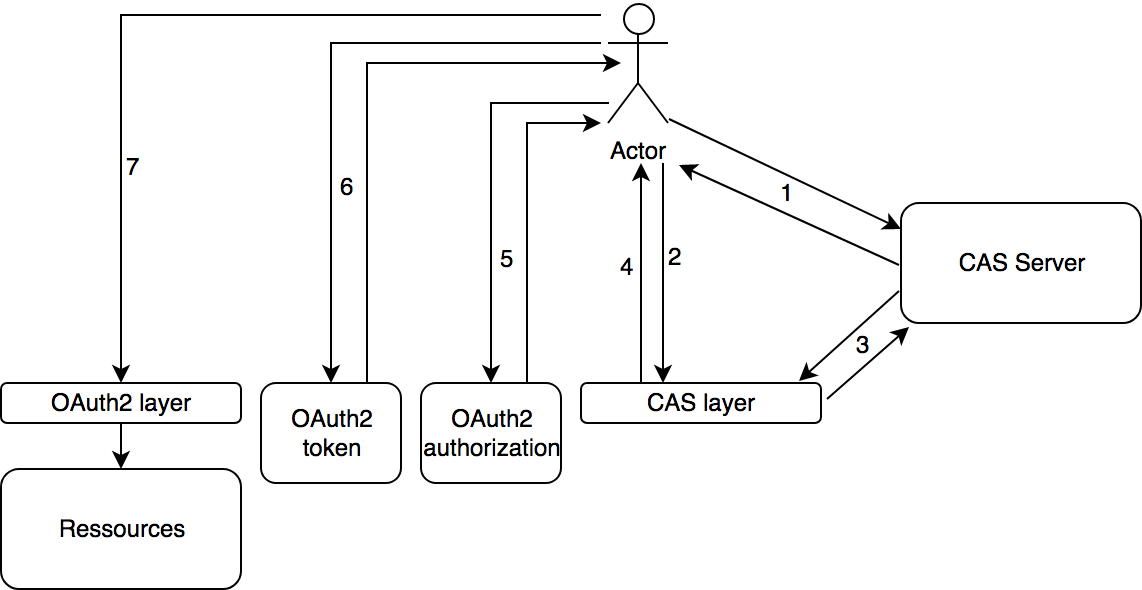
\includegraphics[width=\textwidth]{Figures/modeleAutorisation}
            \begin{tikzpicture}\tikzstyle{every node}=[font=\small]
  \node[bob, minimum size=1.5cm, label={Acteur}] (actor) at (0,0) {};
  \node[draw, rounded corners, inner sep = 0.5cm] (cas_server) at (3,-3) {CAS Server};
  \node[draw, rounded corners, minimum height=2\baselineskip] (cas_layer) at (0,-5) {CAS Layer};
  \node[draw, rounded corners, align=center] (auth) at (-3,-5) {OAuth2 \\ Authorization};
  \node[draw, rounded corners, align=center] (token) at (-6,-5) {OAuth2 \\ Token};
  \node[draw, rounded corners, minimum height = 2\baselineskip] (layer) at (-9,-5) {OAuth2 Layer};
  \node[draw, rounded corners, inner sep=0.5cm] (ress) at (-9,-6.5) {Ressources};
%%%%%%%%%%%%%%%%%
\draw[latex-latex] (cas_server.north west) -- node[midway, fill=white] {1} (actor.south east);
\draw[-latex] (actor.south) -- node[midway, fill=white] {2} (cas_layer);
\draw[latex-latex] (cas_layer.north east) -- node[midway, fill=white] {3} (cas_server.south west);
\draw[-latex] let \p1 = (cas_layer.north), \p2 = (actor.south) in
  ({\x1-12}, \y1) -- node[midway, fill=white] {4} ({\x2-12}, \y2);
\draw[latex-latex] (actor.south west) -- node[midway, fill=white] {5} (auth.north);
\draw[latex-latex] let \p1 = (actor.west) in
  (\x1, {\y1-10}) -- node[midway, fill=white] {6} (token.north);
\draw[latex-latex] let \p1 = (actor.west) in
  (\x1, {\y1+5}) -- node[midway, fill=white] {7} (layer.north);
\draw[-latex] (layer.south) -- (ress.north);
\end{tikzpicture}
            \caption{Modèle d'autorisation implémenté}
            \label{fig.modeleAutorisation}
        \end{figure}  

        \subsubsection{Solutions utilisées}
        \paragraph{Environnement de développement}
        Pour le développement de l'application, la technologie React-Native avec Expo nous a permis une intégration multi-plateforme pour l'environnement de développement. À vrai dire, ces deux technologies nous ont permis de développer efficacement, puisque le code était compilé sur les serveurs d'Expo plutôt que sur la machine du développeur. D'ailleurs, React-Native permet le développement sur Android et iOS en utilisant un unique code source. Comme si ce n'était pas suffisant, Expo nous permet de compiler l'application automatiquement lorsqu'on sauvegarde l'un des fichiers de l'application. Ainsi, nous avons réalisé un environnement de développement applicatif multi-plateforme avec un déploiement mobile Android et iOS en temps réel, ce qui nous a permis d'optimiser notre temps de travail.
        
        \paragraph{Gitlab}
        Le choix de Gitlab a été principalement motivé par la volonté de l'équipe d'utiliser l'intégration et le déploiement continu dans le projet (figure~\ref{fig.gitlab}). Lors de chaque commit, Gitlab faisait un \emph{build} de l'application et roulait les tests. Cela a permis aux développeurs de savoir très rapidement s'ils avaient brisé quelque chose, ce qui est une raison pour refuser un \emph{merge request}. En supplément, pour le serveur, il y avait deux tâches supplémentaires lors de changements dans le \emph{master}. Premièrement, Gitlab faisait une \emph{release}, qui consiste à construire l'image Docker. Ensuite, Gitlab se connectait en SSH sur la machine de production, arrêtait le service, téléchargeait la nouvelle image et repartait le service. Le tout prenait environ une dizaine de minute et nous avions toujours la dernière version à jour sur le serveur de production sans que l'équipe n'ait à s'en soucier.
        
        \begin{figure}[hp] \centering
%            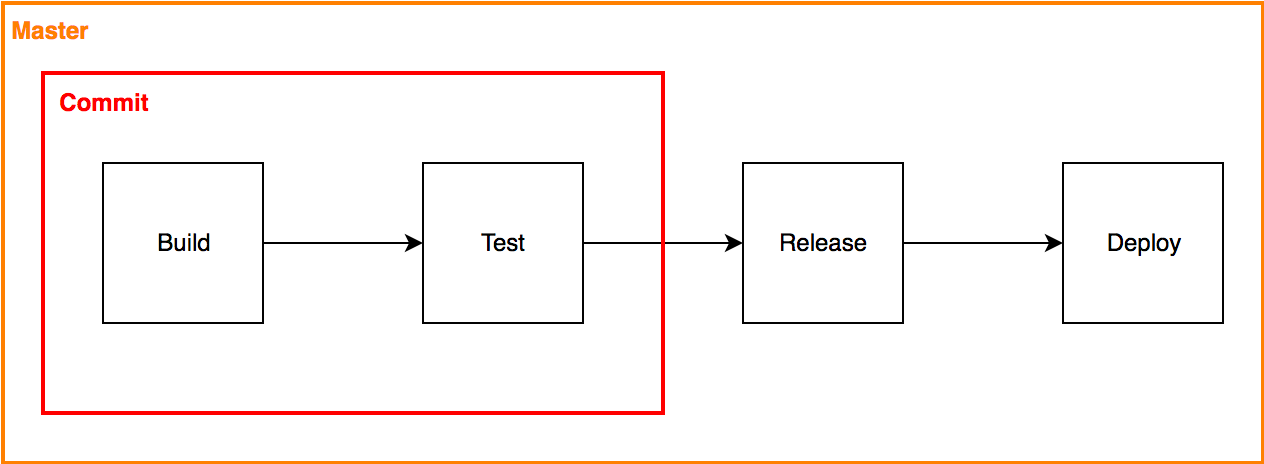
\includegraphics[width=\textwidth]{Figures/gitlab}
            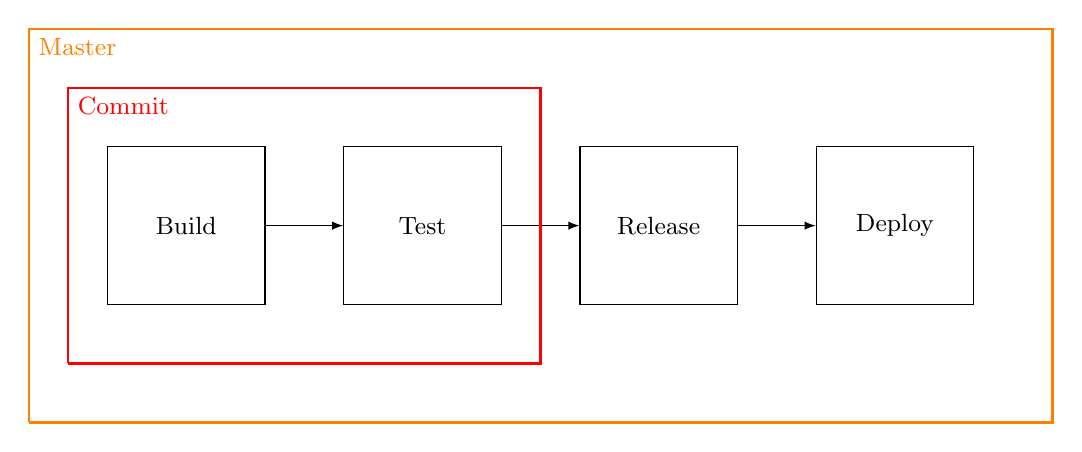
\begin{tikzpicture}\tikzstyle{every node}=[font=\small]
\node[draw, minimum height=2cm, minimum width=2cm] (build) at (0,0) {Build};
\node[draw, minimum height=2cm, minimum width=2cm] (test) at (3,0) {Test};
\node[draw, minimum height=2cm, minimum width=2cm] (release) at (6,0) {Release};
\node[draw, minimum height=2cm, minimum width=2cm] (deploy) at (9,0) {Deploy};
%%%%%%%%%%%%%
\draw[-latex] (build) -- (test);
\draw[-latex] (test) -- (release);
\draw[-latex] (release) -- (deploy);
%%%%%%%%%%%%%
\draw[thick, orange] (-2,-2.5) -- (-2,2.5) -- (11,2.5) -- (11,-2.5) -- (-2,-2.5);
\draw[thick, red] (-1.5,-1.75) -- (-1.5,1.75) -- (4.5,1.75) -- (4.5,-1.75) -- (-1.5,-1.75);
%%%%%%%%%%%%%
\node[anchor=north west, orange] at (-2,2.5) {Master};
\node[anchor=north west, red] at (-1.5,1.75) {Commit};
\end{tikzpicture}
            \caption{Intégration et déploiement continu}
            \label{fig.gitlab}
        \end{figure}  
        
        \paragraph{Docker}
        L'équipe étant très friande de nouvelles technologies, il a été décidé d'utiliser Docker afin d'encapsuler notre serveur Spring (figure~\ref{fig.docker}). Le but est vraiment de créer une boîte noire facile à déployer et qui ne requiert pas de configuration. En plus de cela, l'équipe a utilisé un Docker-Compose afin d'encapsuler l'ensemble des services du backend. Cela crée un réseau virtuel séparé dont le seul point d'entré est un NGINX reverse proxy en HTTPS. Le reste des services peut utiliser des protocoles en clair comme il n'est pas possible d'y accéder de l'extérieur.

        \begin{figure}[hp] \centering
%            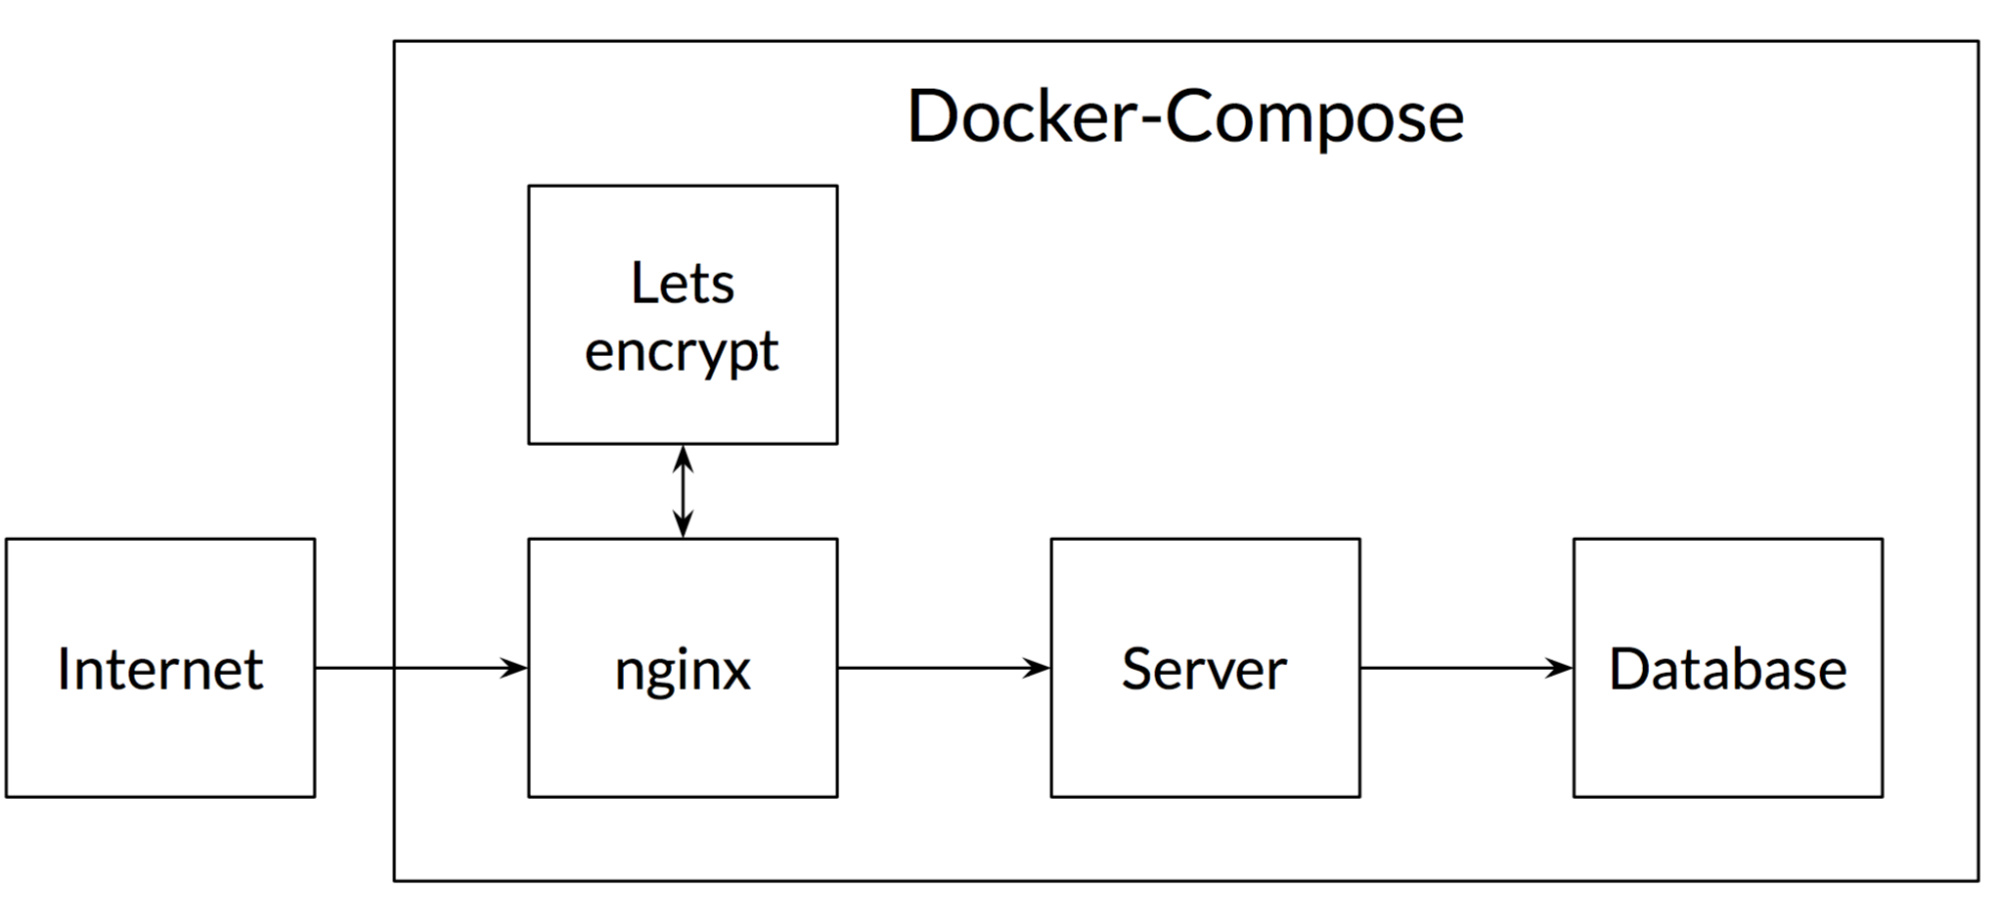
\includegraphics[width=\textwidth]{Figures/docker}
            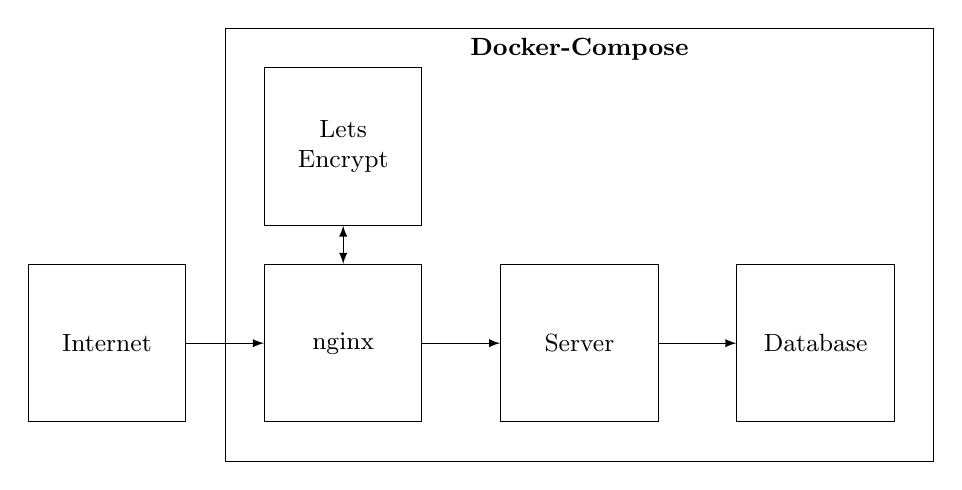
\begin{tikzpicture}
\node[draw, minimum height=2cm, minimum width=2cm] (internet) at (0,0) {Internet};
\node[draw, minimum height=2cm, minimum width=2cm] (nginx) at (3,0) {nginx};
\node[draw, minimum height=2cm, minimum width=2cm] (server) at (6,0) {Server};
\node[draw, minimum height=2cm, minimum width=2cm] (db) at (9,0) {Database};
\node[draw, minimum height=2cm, minimum width=2cm, align=center] (lets) at (3,2.5) {Lets \\ Encrypt};
%%%%%%%%%%%%%
\draw[-latex] (internet) -- (nginx);
\draw[-latex] (nginx) -- (server);
\draw[-latex] (server) -- (db);
\draw[latex-latex] (nginx) -- (lets);
%%%%%%%%%%%%%
\draw (1.5,-1.5) -- (1.5,4) -- node[midway, below] {{\bfseries Docker-Compose}} (10.5,4) -- (10.5,-1.5) -- (1.5,-1.5);
\end{tikzpicture}
            \caption{Services du backend avec Docker-Compose}
            \label{fig.docker}
        \end{figure}

        \paragraph{Spring}
        Spring est le \emph{framework} web Java le plus utilisé mondialement et en entreprise. Il contient énormément d'intégrations (injection de dépendances, CAS, OAuth2, REST, Hibernate, FlywayDB, OpenFeign, etc.) qui nous ont notamment permis d'implémenter notre authentification et notre gestion complexe des permissions sans avoir à ajouter d'autres dépendances externes. La documentation et le support sont également excellents puisque la communauté est très vaste et active.
        
        \paragraph{Kotlin}
        Kotlin est un langage récent développé par JetBrains qui roule sur la JVM. Sa grande force est qu'il est interopérable à 100~\% avec Java, ce qui nous a permis d'utiliser toutes les libraires déjà présentes dans l'écosystème Java. Un peu comme le Java depuis la version 8, Kotlin est un langage qui est influencé par le fonctionnel tout en gardant une forte base orientée-objet. De plus, le langage est \emph{null-safe} et emprunte beaucoup de concepts d'immuabilité, ce qui le rend très sécuritaire. Finalement, le langage possède une syntaxe moderne et est peu verbose, ce qui le rend très agréable à utiliser. Pour toutes ces raisons, l'entièreté du backend a été codée avec Kotlin.

        \paragraph{Intégration Horarius}
        Par défaut, l'utilisation d'\emph{Horarius} n'a pas d'API en place pour la détection d'un changement à l'horaire. Nous avons solutionné ce problème à l'aide d'un ajout de fonctionnalité dans le backend qui différencie les horaires à chaque 5~minutes. Plus précisément, chaque étudiant utilise un lien iCal dont l'horaire complet peut être téléchargé. En émettant ce lien iCal, nous avons évalué l'évolution de chaque horaire dans un intervalle de temps. De manière optimale, l'intégration de cette vérification doit être conçue à partir de l'administration des horaires puisque chaque requête de téléchargement au serveur de l'université est lourde et demande beaucoup de bande passante pour une simple application. Nous avons donc une solution pour la preuve de concept, et il suffirait d'un engagement plus concret de la part du service d'administration des locaux de l'université pour optimiser le processus.

        \paragraph{Notification}
        Lorsqu'une information pertinente doit être communiquée à l'utilisateur, le système de notifications de Facebook propose un moyen efficace pour l'envoi de notifications. Ces alertes peuvent devenir très complexes à gérer puisque la diversité du type de notifications, la compatibilité multi-plateforme et la permissivité sont des facteurs influençant la qualité du sous-logiciel. Dans l'optique d'une meilleure efficacité, on utilise le système de notifications de Facebook, qui gère très bien les notifications pour plusieurs raisons : multi-plateforme, simple d'utilisation, exemplifié concrètement et pré-configuré pour Expo.
    
    \subsection{Problèmes rencontrés}
    L'un des problèmes rencontrés lors du développement mobile est le manque de documentation pour la technologie Expo. À vrai dire, les exemples d'application mobile Expo similaires sur le web ont été plus bénéfiques pour l'avancement du logiciel que la documentation en soi. D'ailleurs, une étude sur la technologie React-Native estime que le temps passé à écrire le code React-Native est inférieur à 1~\%, \cite{react}. React native propose donc un moyen simple d'intégration et de compatibilité multiplateformes, mais ce travail est un casse-tête constant pour les débutants.

    \begin{figure}[hp] \centering
%        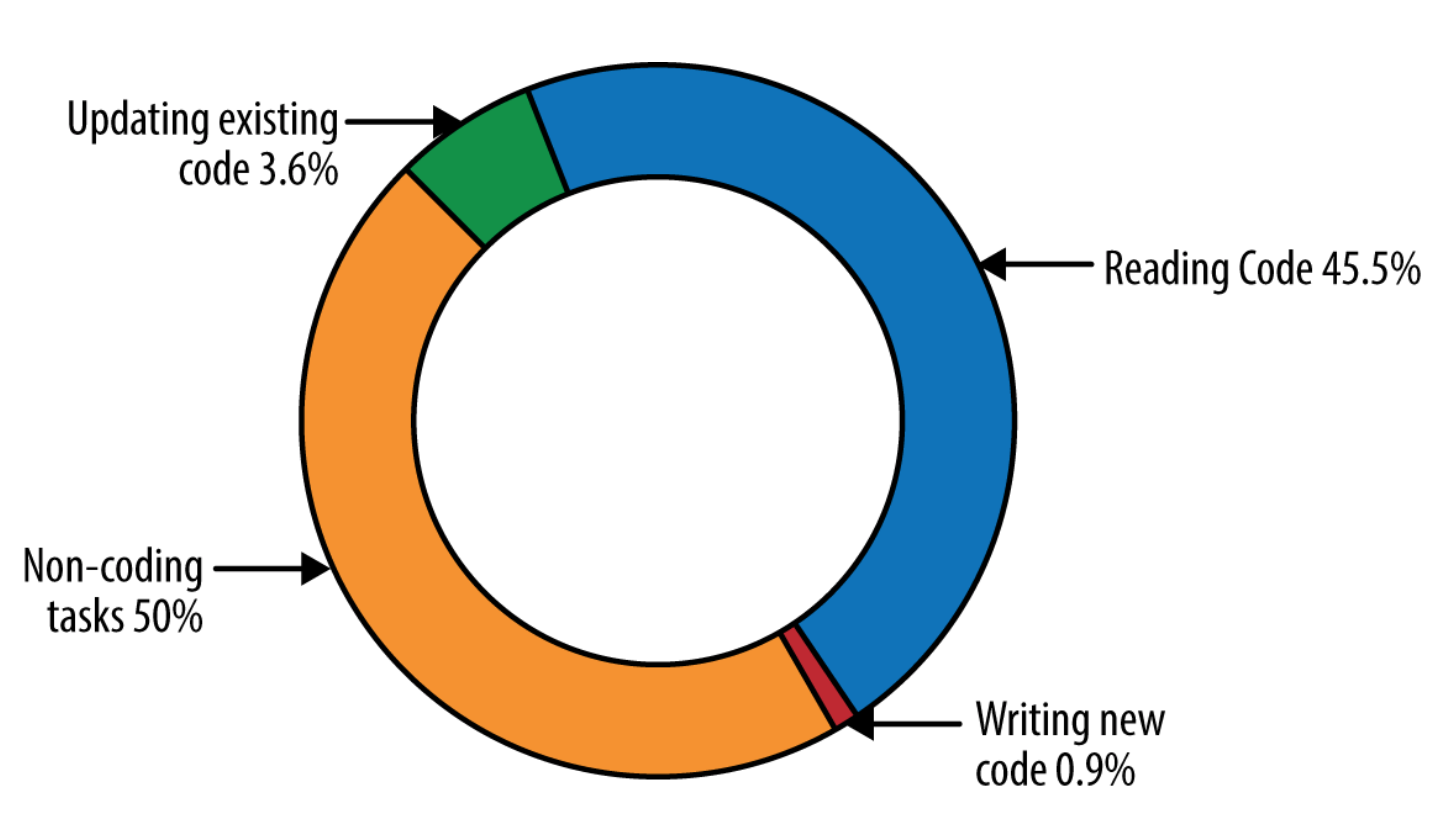
\includegraphics[width=\textwidth]{Figures/react}
        \definecolor{newRed}{HTML}{C12932}
\definecolor{newOrange}{HTML}{F79232}
\definecolor{newBlue}{HTML}{0273B9}
\definecolor{newGreen}{HTML}{049148}
%
\wheelchart{3.6/newGreen/{Updating existing code},  50/newOrange/{Non-coding tasks}, 0.9/newRed/{Writing new code}, 45.5/newBlue/{Reading code}}
        \caption{Répartition du temps dans un projet React Native}
        \label{fig.react}
    \end{figure}
    
    Comme mentionné précédemment, l'absence d'API pour la notification lors d'un changement à l'horaire a été un problème important pendant le développement. Tout d'abord, nous avons tenté de résoudre ce manque avec le groupe professoral, mais en vain. Voyant l'échéancier arriver à grands pas, nous avons décidé de concevoir notre propre logique d'évaluation de changement temporelle d'horaire. Évidemment, cela a généré d'autres problèmes connexes à cet ajout de fonctionnalité. Entre autres, le temps de calcul et la bande passante disponible sont inévitablement des paramètres qui ont été analysés pendant la conception.
    
    Finalement, nous avons rencontré de nombreux problèmes lors de la mise en \oe{}uvre de l'authentification. En effet, personne ne fait ce genre d'authentification CAS et OAuth2, car c'est redondant. On choisit généralement l'un ou l'autre et/ou on a le contrôle sur le serveur d'authentification. Il a fallu lire de nombreux tutoriels et expérimenter longtemps pour arriver à une solution fonctionnelle et sécuritaire. Nous avons même écrit un document technique assez poussé détaillant précisément comment CAS et OAuth2 fonctionne en général et dans l'application afin de garder une trace de nos recherches.
